\begin{figure*}[t]
\centering
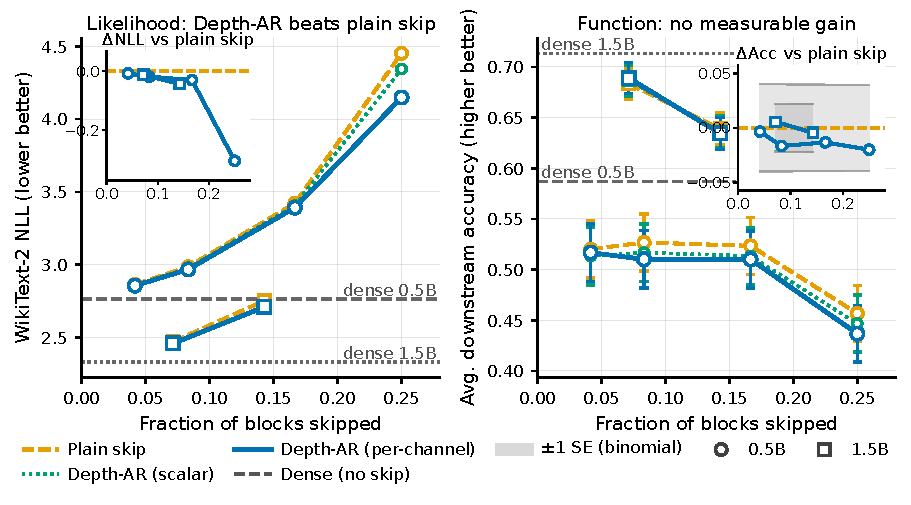
\includegraphics[width=0.62\textwidth]{figures/fig2_dissociation.pdf}
\caption{\textbf{Prediction pays off in proportion to what skipping destroys.} Quality against
the fraction of blocks skipped for Qwen2.5-0.5B (circles), 1.5B (squares) and 7B (triangles),
layers chosen by measured residual damage, the deployable rule, with every predictor skipping
the identical blocks. Bands are binomial standard error with the measured 0.44-point
harness jitter folded in quadrature (\Cref{sec:app-noise}); the lighter outer band is
$1.96$~SE. Where skipping barely hurts, at the left of each panel, \mname and plain skipping
are indistinguishable in behaviour, and the differences there lie below the evaluation's own
reproducibility floor. Where skipping does severe damage the gap opens: at 28.6\% of
blocks skipped on 7B, \mname answers 89 more questions correctly out of 900 than
plain skipping ($z=4.31$, surviving Bonferroni correction across all 63
comparisons) while recovering 38.1\% of its language-modelling damage. Both breakdowns
are drawn rather than hidden: at 42.9\% skipped on 7B the depth-only predictor falls
\emph{below} plain skipping on likelihood, where the cross-token extension of
\Cref{sec:app-crosstoken} does not. Hardware and protocol: \Cref{sec:app-protocol}.}
\label{fig:dissociation}
\end{figure*}
